% word limit: 500
\section{Results and Discussion}
\label{sec:results}

% \subsection{Velocity dispersion of coeval groups}
% \label{sec:age_cut}

% To explore the relationship between rotation period, \teff\ and age for field
% K dwarfs, we calculated gyrochronal ages using dereddened \Gaia\ photometry
% ($G$, $G_{BP}$ and $G_{RP}$) and rotation periods from \citet{mcquillan2014}.
% We used the \citet{angus2019} gyrochronology relation which is a simple,
% separable relation in \gcolor\ color and age, calibrated using the
% period-color relation of Praesepe and the period-age relation of Praesepe and
% the Sun.
% The large number of Praesepe members with precise rotation periods from the
% \ktwo\ mission \citep{howell2014, douglas2017, rebull2017}, spanning spectral
% types F through early M, makes it a good cluster for calibrating the
% period-color relation of stars at young ages.
% However, this is an extremely simple model and although it accurately
% describes the rotation periods of F and G stars up to around 2.5 Gyr (the age
% of NGC 6819 -- the oldest cluster with available rotation periods), it
% over-predicts the rotation periods of K dwarfs in the 1.1 Gyr NGC 6811
% cluster.

% We then selected groups of stars within different gyrochronal age ranges and
% calculated the standard deviation of \vb\ velocities (\sigmavb), as a function
% of effective temperature for each age group.
% Ages were calculated using dereddened \gaia\ \gcolor\ color, however
% throughout this paper we show rotation periods as a function of effective
% temperature, \teff, because it is easier to divide stars into bins of roughly
% equal numbers in \teff-space than in color-space.

% \begin{figure}
%   \caption{
% Top: rotation period vs effective temperature for stars in the \mct\
%     catalog.
%     The full catalog, with subgiants and visual binaries removed is shown in
%     grey, and stars selected to be in different age groups (between \tmin\ and
%     \tmax\ K) are overlayed in color.
% These age groups were selected using the \citet{angus2019} gyrochronology
%     relation.
% The legend in the center of the figure lists the age range, in Gyr, of each
%     group.
% Bottom: velocity dispersion vs effective temperature for each age
%     group.
% The color of the line corresponds to the color of the group shown in the top
%     panel.
% If the gyrochronal model were correct at all ages, and the stars in each group
%     were the same age across temperatures, the velocity dispersion would be
%     constant as a function of \teff.
% However, the velocity dispersions of the oldest age groups increase with
%     \teff, indicating the \citet{angus2019} gyrochronology model underpredicts
%     the the ages of late-K dwarfs relative to the ages of late G and early K
%     dwarfs at old ages.
% % An alternative explanation could be that the gyrochronology relation is
% %     correct and {\it mass-dependent heating} is responsible for the greater
% %     velocity dispersions of cooler stars.
% }
%   \centering
%     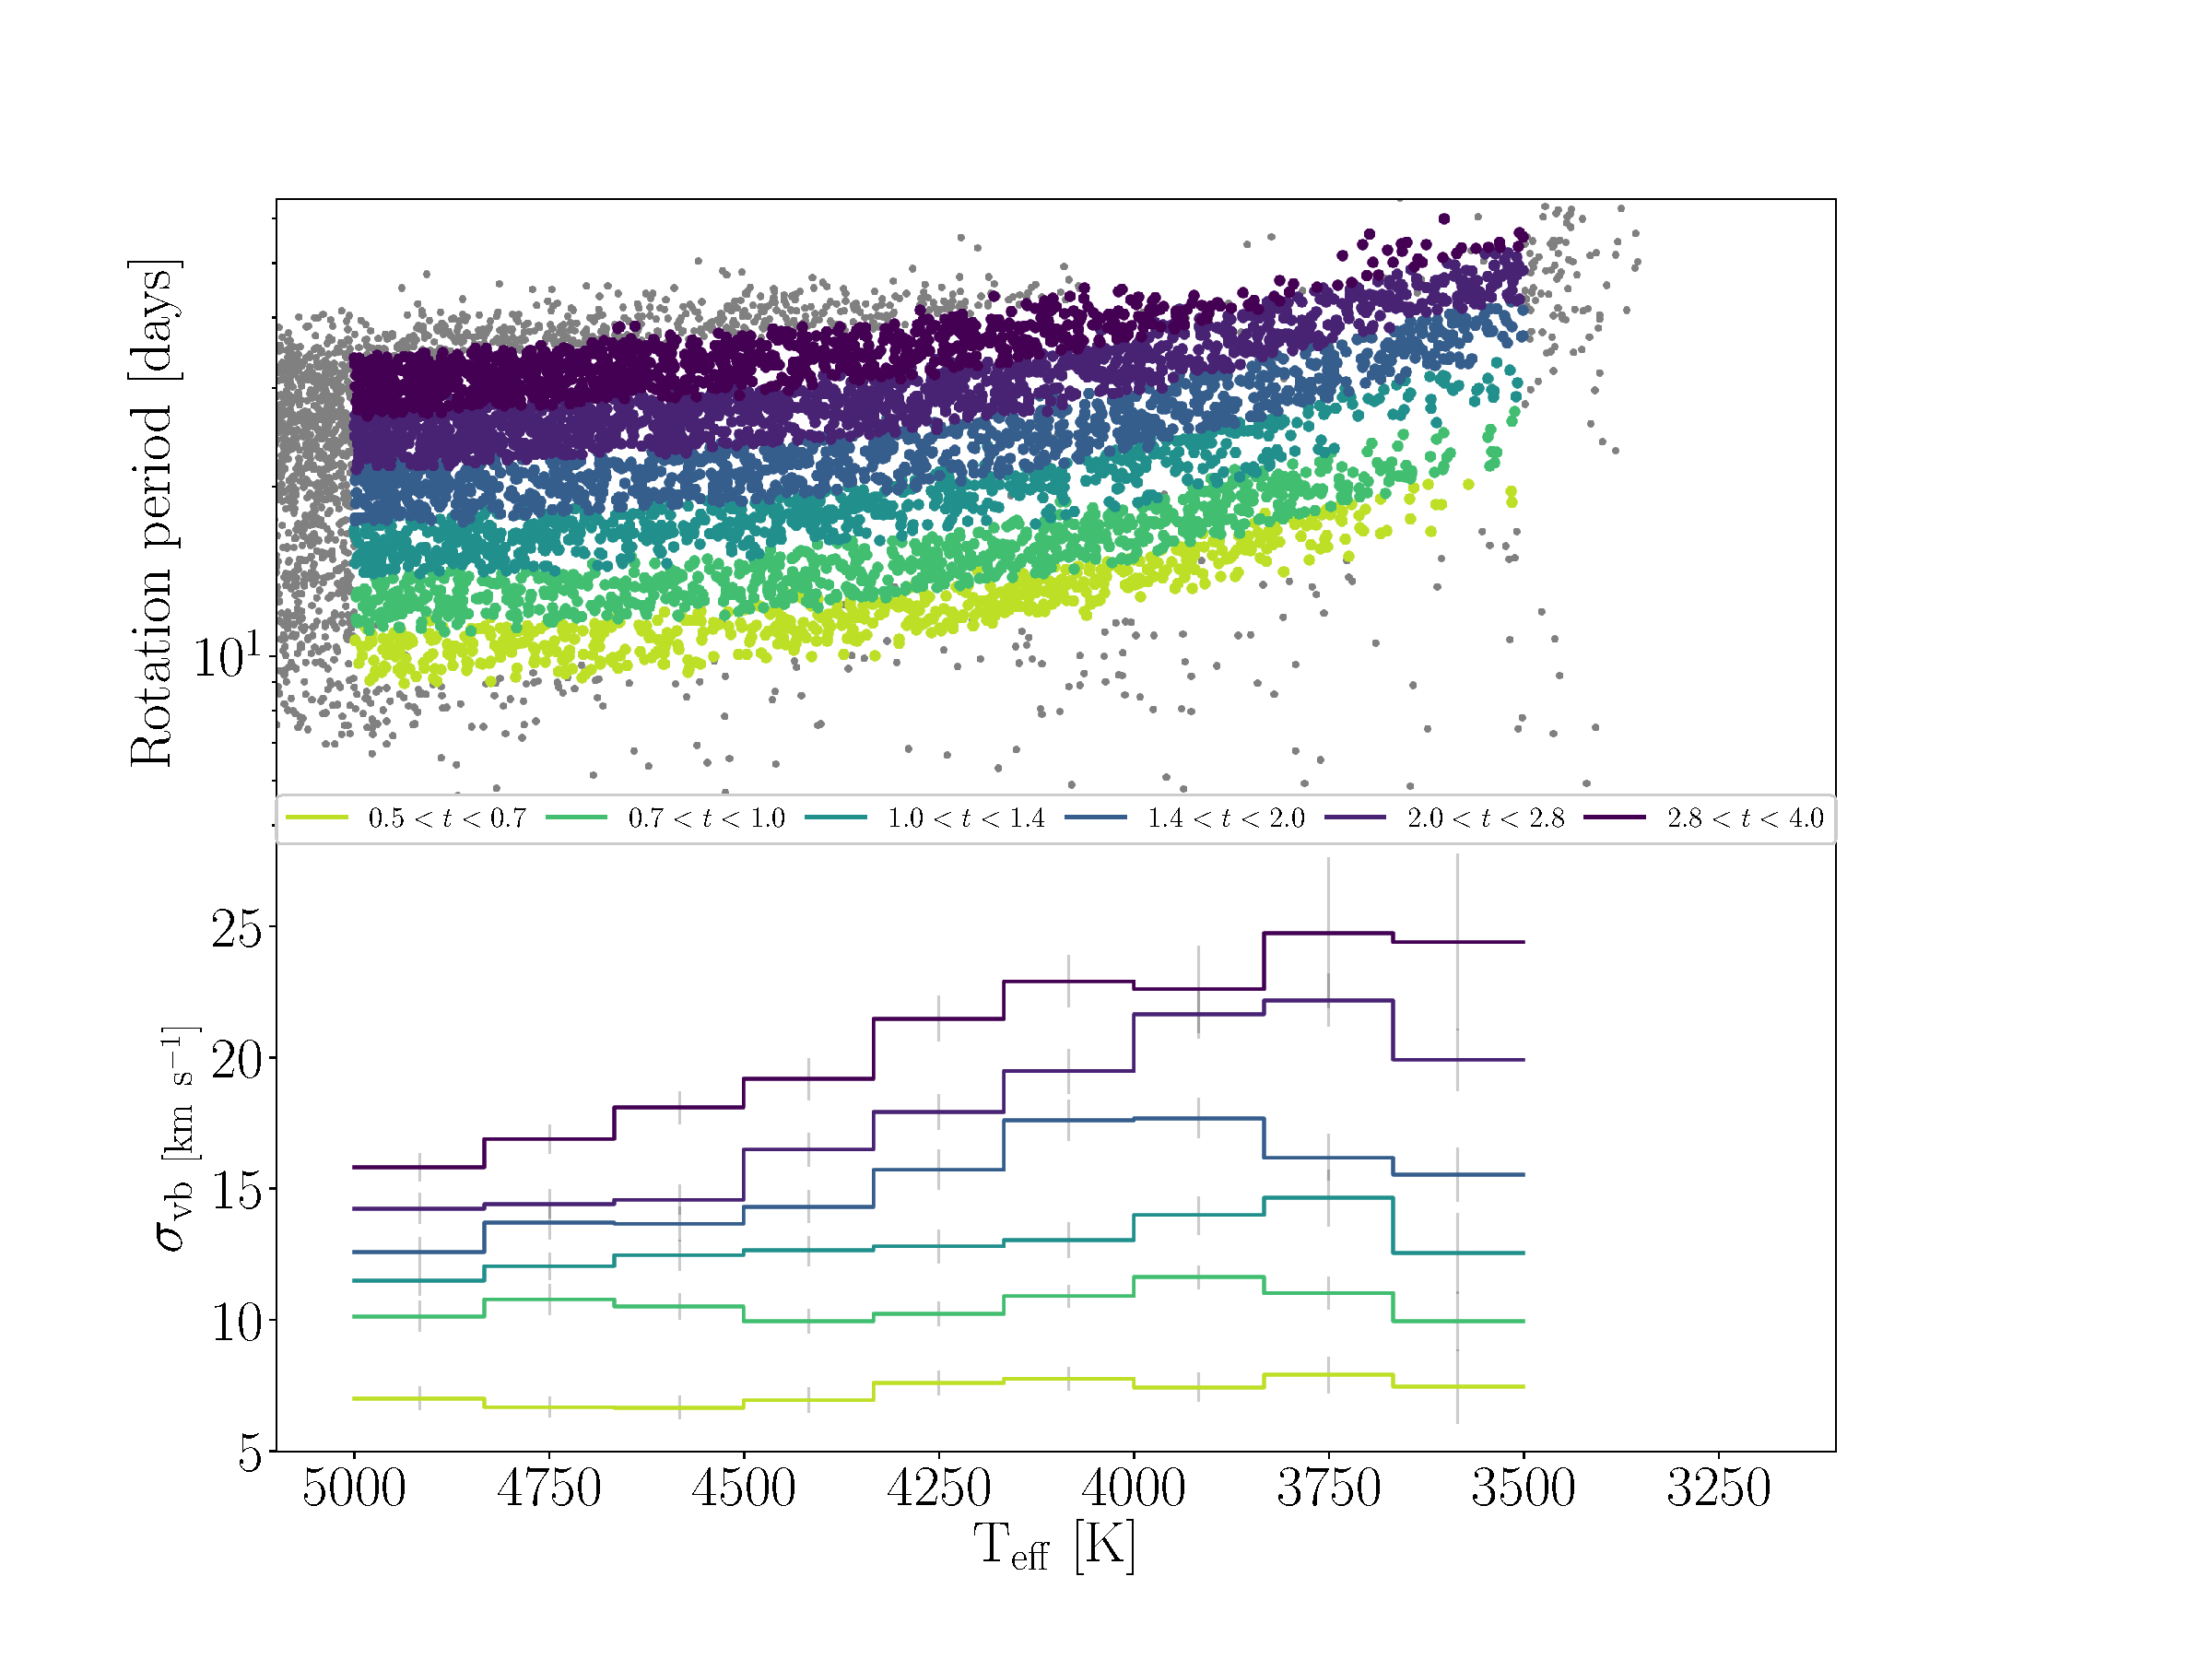
\includegraphics[width=1\textwidth]{age_cut}
% \label{fig:age_cut}
% \end{figure}
% The top panel of figure \ref{fig:age_cut} shows the full \mct\ sample
% (excluding visual binaries and subgiants) in grey, with coeval groups
% \citep[according to the][relation]{angus2019} shown in color.
% The color of the points corresponds to the age ranges specified in the legend
% (in Gyr), which also apply to the lines in the lower panel.
% The bottom panel shows the velocity dispersion, \sigmavb\ of each age group,
% as a function of effective temperature.
% % We only included stars within a temperature range of 5000 - 3500 K in our
% % analysis, as hotter stars are more likely to have stopped magnetic braking
% % \citep{vansaders2016}, which could bias the results.
% % Late M dwarfs were not included in our analysis because such faint stars
% % cannot be observed at large heights above the plane (because of the low
% % galactic latitude of the \kepler\ field, stars at high-Z are more distant),
% % which introduces a mass-dependent velocity bias: cooler populations of stars
% % are skewed towards lower velocity dispersions.
% % The coolest temperature bins in the lower panel of figure \ref{fig:age_cut}
% % have low velocity dispersions, indicating that this effect may already become
% % important at temperatures lower than $\sim$ 4000 K.
% Overall, figure \ref{fig:age_cut} shows that velocity dispersion increases
% with gyrochronal age across all temperatures, implying that both velocity
% dispersion and rotation period increases with age as expected.
% The flat velocity dispersion of young stars as a function of temperature
% shows that the Praesepe-calibrated gyrochronology relation accurately predicts
% the relative ages of {\it young} field stars.
% % To our knowledge, no gyrochronology relation has previously been demonstrated to
% % correctly predict ages (either relative or absolute) for such cool or such
% % young field stars.
% % This is not particularly remarkable however, since these young stars are a
% % similar age to the Praesepe cluster, which was used to calibrate the
% % period-color relation.
% % However, if the stars in each selected age group had the {\it same} age across
% % the temperature range, their velocity dispersion would be a constant function
% % of \teff.
% If \citet{angus2019} gyrochronology relation worked at all ages and
% temperatures, the bottom panel of figure \ref{fig:age_cut} would show a flat
% relationship between velocity dispersion and \teff at all ages.
% However, velocity dispersion {\it increases} as a function of temperature for
% old stars, meaning the \citet{angus2019} gyrochronology relation either
% under-predicts the ages of old, late-K dwarfs, or over-predicts the ages of
% old early-K and late-G dwarfs\footnote{Since \vb\ velocity dispersion only
% provides relative and not absolute ages, it is difficult to tell whether the
% ages of cool stars are being under-predicted, the ages of hot stars being are
% over-predicted, or both.}.
% This suggests that the relationship between rotation period and photometric
% color or \teff\ flattens out over time, and possibly even inverts.
% % The lines of constant age (isochrones) sweeping diagonally upwards in the top
% % panel of figure \ref{fig:age_cut} are too steeply sloped at old ages.

\subsection{The period-\teff\ relations, revealed}
\label{sec:the_reveal}

To explore the relationship between rotation period, \teff\ and velocity
dispersion, we first removed high and low velocity outliers from the \mct\
sample by performing 3$\sigma$ sigma-clipping on the \vb\ velocities.
Without sigma-clipping, we found that a small number of high velocity
outliers at the low-temperature end of our sample substantially raised the
velocity dispersion for cooler stars, however the overall trends remain the
same without sigma-clipping.
% We also limited the sample to temperatures in the range 6000 K $<$ \teff\ $<$
% 3500 K to avoid biases caused by the selection function at the faint, cool
% end, and binarity or weakened braking \citep{vansaders2016} at the hot end.
Finally, we removed stars with rotation periods shorter than the bulk of
periods, since this area of the period-\teff\ diagram is sparsely populated.
We removed rapid rotators by cutting out stars with gyrochronal ages less than
0.5 Gyr, because a 0.5 Gyr gyrochrone\footnote{A gyrochrone is a
gyrochronological isochrone, or a line of constant age in period-\teff, or
period-color space.} traces the bottom edge of the main population of rotation
periods.
After these cuts, 6879 stars were included in the sample.

The top panel of figure \ref{fig:vplot} shows rotation period versus effective
temperature for the \mct\ sample, coloured by the standard deviation of their
(\vb) velocities, where \sigmavb\ was calculated for groups of stars over a
grid in $\log_{10}$(period) and temperature.
If we assume that mass dependent heating does not strongly affect this sample
and \vb\ at low galactic latitudes is an unbiased tracer of \vz, then \vb\
velocity dispersion can be interpreted as an age proxy, and stars plotted in a
similar color in figure \ref{fig:vplot} are similar ages.
\begin{figure}
  \caption{
    Top: Rotation period vs effective temperature for stars in the \mct\
    sample, colored by the velocity dispersions of stars calculated over a
    grid in $\log_{10}$(period) and \teff.
    Black lines show gyrochrones from a gyrochronology model that projects the
    rotation-color relation of
    Praesepe to longer rotation periods over time \citep{angus2019}.
    These gyrochrones do not appear to reflect the evolution of field stars at
    long rotation periods/old ages because they do not trace lines of constant
    velocity dispersion.
    Gyrochrones are plotted at 0.5, 1, 1.5, 2, 2.5, 4 and 4.57 Gyr in both top
    and bottom panels.
    Bottom: Same as top panel with rotation period vs {\it mass}
    \citep[from][]{berger2020}.
    White lines show gyrochrones from a model that includes mass and
    age-dependent angular momentum transport between the core and envelope
    \citep{spada2019}.
    Qualitatively, these gyrochrones reflect the evolution of field
    stars at long rotation periods/old ages: they trace lines of constant
    velocity dispersion by reproducing periods of `stalled' rotational
    evolution for K-dwarfs.
}
  \centering
    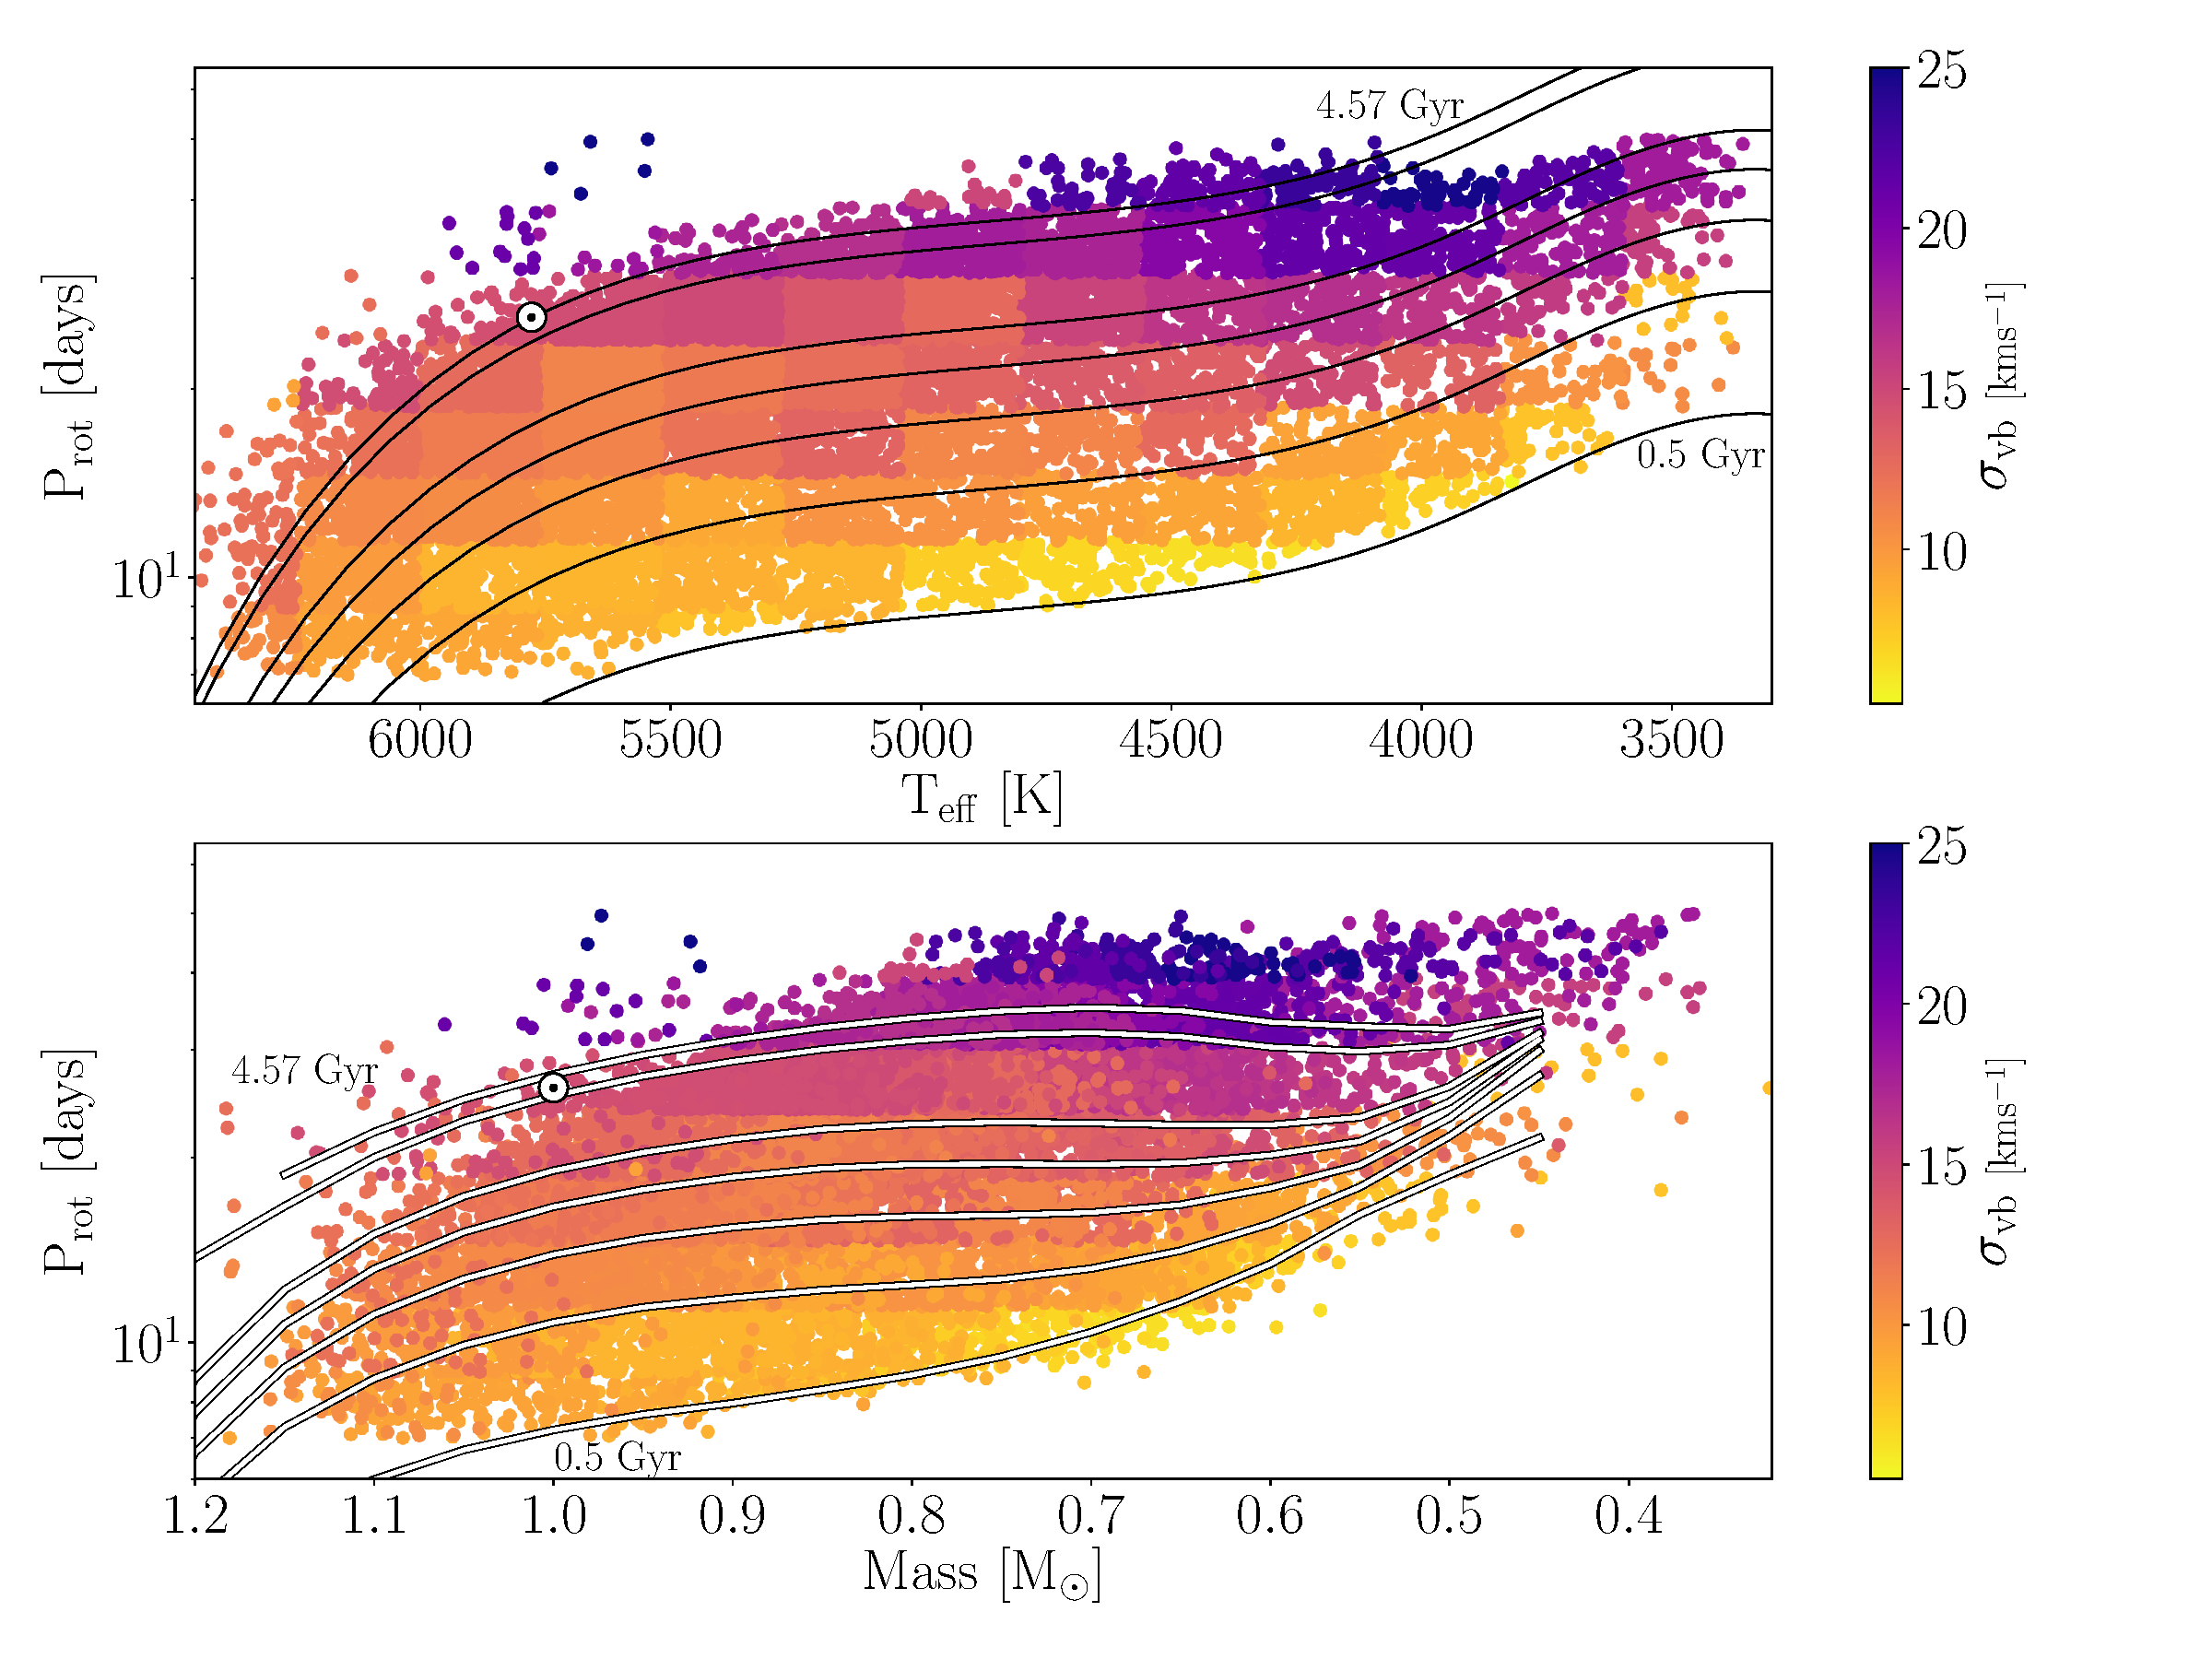
\includegraphics[width=1\textwidth]{main_figure}
\label{fig:vplot}
\end{figure}
Overall, figure \ref{fig:vplot} shows that velocity dispersion increases with
rotation period across all temperatures, implying that rotation period
increases with age, as expected.
This result is insensitive to the choice of bin position and size.
Black lines show gyrochrones from the \citet{angus2019} gyrochronology model,
which projects the rotation-color relation of Praesepe to longer rotation
periods over time.
These gyrochrones are plotted at 0.5, 1, 1.5, 2, 2.5, 4 and 4.57 Gyr.
At the youngest ages, these gyrochrones describe the data well: the palest
yellow (youngest) stars with the lowest velocity dispersions all fall close to
the 0.5 Gyr gyrochrone.
% Lines of constant age (isochrones) appear to follow the shape of the
% Praesepe-based gyrochronology model (black dotted line) at young ages.
% However, at older ages it appears that the relation between rotation period
% and \teff\ flattens out, until eventually rotation period {\it decreases} with
% decreasing effective temperature at a given age.
However, although the 0.5 Gyr and 1 Gyr gyrochrones also trace constant
velocity dispersion/age among the field stars, by 1.5 Gyr the gyrochrones
start to {\it cross} different velocity dispersion regimes.
For example, the 1.5 Gyr gyrochrone lies on top of stars with velocity
dispersions of around 10-11 kms$^{-1}$ at 5000-5500K and stars with $\sim$15
\kms\ velocity dispersions at 4000-4500K.
The gyrochrones older than 1.5 Gyr also cross a range of velocity dispersions.
If these were true isochrones they would follow lines of constant velocity
dispersion.
At ages older than around 1 Gyr, it appears that gyrochrones should have a more
flattened, or even inverted relationship between rotation period and effective
temperature than these Praesepe-based models.
% For late K-dwarfs older than around 1 Gyr, it appears that lower-mass stars
% rotate more rapidly than higher-mass stars.
% This is the opposite of the trend that is observed in young open clusters such
% as Praesepe and the Hyades.

The bottom panel of figure \ref{fig:vplot} shows velocity dispersion as a
function of rotation period and {\it mass}, \citep[from][]{berger2020}, with
gyrochrones from the \citep{spada2019} model shown in white.
These gyrochrones are also plotted at 0.5, 1, 1.5, 2, 2.5, 4 and 4.57 Gyr.
Each point plotted in the top panel also appears in the bottom panel with the
same color.
Because velocity dispersion was calculated in bins of \teff, not mass, bin
outlines are clearly visible in the top panel but appear smeared-out in the
bottom panel.
In the bottom panel of figure \ref{fig:vplot}, the \citet{spada2019} models
{\it do} trace lines of constant velocity dispersion, and reproduce the trends
in the data at all ages.
These models qualitatively agree with the data and reproduces the apparent
flattening and inversion in the rotation period-\teff/mass relations.

The results shown in figure \ref{fig:vplot} indicate that stars of spectral
type ranging from late G to late K ($\sim$5500-3500 K) follow a braking law
that changes over time.
In particular, the relationship between rotation period and effective
temperature appears to flatten out and eventually invert.
These results provide further evidence for `stalled' rotational evolution of K
dwarfs, like that observed in open clusters \citep{curtis2019} and reproduced
by models that vary angular momentum transport between stellar core and
envelope with time and mass \citep{spada2019}.
The velocity dispersions of stars in the \mct\ sample provide the following
picture of rotational evolution.
At young ages \citep[younger than around 1 Gyr but still old enough to be on
the main sequence and have transitioned from the `I' sequence to the `C'
sequence ][]{barnes2003}, stellar rotation period decreases with increasing
mass.
This is likely because lower-mass stars with deeper convection zones have
stronger magnetic fields, larger Alfv\'en radii and therefore experience
greater angular momentum loss rate.
According to the \citet{spada2019} model, there is minimal transportation of
angular momentum from the surface to the core of the star at these young ages,
so the surface slows down but the core keeps spinning rapidly.
At intermediate ages, rotation period is constant with mass, and at late ages
rotation period {\it increases} with mass for K-dwarfs.
The interpretation of this, according to the \citet{spada2019} model, is that
lower-mass stars are still braking more efficiently at these intermediate and
old ages but their cores are more tightly coupled to their envelopes, allowing
angular momentum transport between the two layers.
Angular momentum resurfaces and prevents the stellar envelopes from
spinning-down rapidly, and this effect is strongest for late K-dwarfs with
effective temperatures of $\sim$4000-4500K and masses $\sim$0.5-0.7 M$_\odot$.

It has been demonstrated that lower-mass stars remain magnetically active
longer than more massive stars, \citep[\eg][]{west2008, kiman2019}.
If the detectability of a rotation period is considered to be a magnetic
activity proxy, then our results provide further evidence for a mass-dependent
activity lifetime.
Figure \ref{fig:vplot} shows that the groups of stars with the largest
velocity dispersions are cooler than 4500 K.
This implies that the oldest stars with detectable rotation periods, are
cooler than 4500 K, \ie\ these-low mass stars stay active longer than more
massive stars.

\subsection{The period gap and synchronized binaries}
\label{sec:gap}

There is a sharp gap in the population of rotation periods, which lies just
above the 1 Gyr gyrochrone in the upper panel of figure \ref{fig:vplot}, whose
origin is unknown and is the subject of much speculation \citep{mcquillan2014,
davenport2018, reinhold2019}.
The Praesepe-based model appears to be valid below the gap but not above.
Although this may be coincidental (and more data would be needed to confirm a
connection) the gap may indeed separate a young regime where stellar cores are
decoupled from their envelopes from an old regime where these layers are more
tightly coupled.
If so, this could indicate that the phenomenon responsible for changing the
shape of gyrochrones in rotation-\teff\ space is related to the phenomenon that
produces the gap.

\begin{figure}
  \caption{
      Top: rotation period vs. effective temperate for stars in the \mct\
    sample, separated into three groups. Blue circles
      show stars with rotation periods longer than the
    period gap, orange squares show stars with rotation periods shorter than
    the gap, but longer than the lower edge of the main rotation period
    distribution, and green triangles show stars with rotation periods shorter
    than this lower edge.
    Stars were separated into these three groups using \citet{angus2019}
    gyrochronology models, with the scheme shown in the legend.
    Only stars cooler than 5000 K are plotted in
    the bottom panel in order to isolate populations above and below the
    period gap, which only extends up to temperatures of $\sim$4600 K.
    Bottom: the velocities of these groups of stars (in the direction of
    Galactic latitude, $b$) are shown as a function of rotation period.
    The black line indicates the velocity standard deviation as a function of
    period.
}
  \centering
    \includegraphics[width=1\textwidth]{gap}
\label{fig:gap}
\end{figure}

The bottom panel of figure \ref{fig:gap} shows the velocity dispersions of
stars in the \mct\ sample, with stars subdivided into three groups: those that
rotate more quickly than the major rotation period distribution (green
triangles), those with rotation periods shorter than the gap (orange squares),
and those with rotation periods longer than the gap (blue circles).
Stars were separated into these three groups using \citet{angus2019}
gyrochronology models, according to the scheme shown in the legend.
Only stars cooler than 5000 K are included in the bottom panel in order to
isolate populations above and below the period gap, which only extends up to a
temperature of $\sim$4600 K in our sample \citep[Although][found that the gap
extends to temperatures as hot as 6000 K]{davenport2017}.
In general, velocity dispersion increases with rotation period because both
quantities increase with age.
There is a smooth transition in velocity dispersion between stars with
rotation periods below and above the gap (orange squares to blue circles),
suggesting that these groups are part of the same galactic population.
Previously, only the overall velocity dispersions of all stars above and below
the gap have been compared, leading to the assumption that these groups belong
to two distinct populations \citep{mcquillan2014}.
On the other hand, the velocity dispersions of stars with rotation periods
shorter than the lower edge of the rotation period distribution (green
triangles) are not significantly smaller than the, presumed older,
orange-colored stars.
% This is an indication that many of these are synchronized binaries.
% The rotation periods of stars in synchronized binaries are tidally locked to
% the orbital period of the binary system and since synchronized binaries have
% short orbital periods this can produce old, seemingly isolated stars, with
% short rotation periods.
The large velocity dispersions of the most rapidly rotating stars indicates
that some fraction of these stars are old but rotating rapidly, and therefore
likely to be synchronized binaries.
% Given the strong correlation between binary fraction and primary mass
% \citep[\eg][]{price-whelan2020}, and the fact that M dwarfs take longer to
% transition from the `I` (rapidly rotating) sequence to the `C' (slowly
% rotating) sequence, it is likely that
Figure \ref{fig:gap} indicates that there is an increased probability of stars
with rotation periods less than $\sim$10 days being synchronized binaries.
This result is in agreement with a recent study which found that a large
fraction of photometric binaries were rapid rotators, and the probability of a
star being a synchronized binary system substantially increased below rotation
periods of around 7 days \citep{simonian2019}.

\subsection{Validating \vb\ dispersion as an age proxy}
\label{sec:mass-dependent-heating}

There are two main reasons why \vb\ velocity dispersion may not be a good age
proxy.
Firstly, mass-dependent heating may act on the sample, meaning that velocity
dispersion depends on both age and mass, so cannot be interpreted as a simple
age proxy.
Secondly, since stars in the \kepler\ field have a range of galactic
latitudes, using \vb\ as a stand-in for \vz\ may not be equally valid for all
stars, and introduce a velocity bias for high latitude stars (which are more
likely to be cooler and older).
In this section we demonstrate that neither of these problems seem to be a
significant issue for our data.

In order to establish whether \sigmavb\ can be used as an age proxy, we
searched for signs of mass-dependent heating within the \kepler\ field.
Mass-dependent dynamical heating may result from lower-mass stars experiencing
greater velocity changes when gravitationally perturbed than more massive
stars.
It has not been unambiguously observed in the galactic disk because of the
strong anti-correlation between stellar mass and stellar age.
Less massive stars do indeed have larger velocity dispersions, however they
are also older on average.
This mass-age degeneracy is highly reduced in M dwarfs because their
main-sequence lifetimes are longer than the age of the Universe, and no
evidence for mass-dependent heating has previously been found in M dwarfs
\citep[\eg][]{faherty2009, newton2016}.

To investigate whether mass-dependent heating could be acting on the \kepler\
sample, we selected late K and M dwarfs observed by both \kepler\ and \gaia,
whose MS lifetimes exceed around 11 Gyr and are therefore representative of
the initial mass function.
We could not perform this analysis on the \mct\ sample, because it only
includes stars with {\it detectable} rotation periods, and since lower-mass
stars stay active for longer it is likely that it contains a strong mass-age
correlation.
We selected all \kepler\ targets with dereddened \gaia\ \gcolor\ colors
greater than 1.2 (corresponding to an effective temperature $\lesssim$
4800 K) and absolute \gaia\ $G$-band magnitudes $<$ 4.
We also eliminated photometric binaries by removing stars above a 6th order
polynomial, fit to the MS on the \gaia\ CMD (similar to the one shown in
figure \ref{fig:age_gradient}).
We then applied the quality cuts described above in section
\ref{sec:the_data}.
To search for evidence of mass-dependent heating we calculated the (\vb)
velocity dispersion of stars in effective temperature bins.
Sigma clipping was performed at 3$\sigma$ to remove high and low velocity
outliers before calculating the standard deviation of stars in each bin.
These extreme velocity outliers may be very old late K and M dwarfs, or they
result from using \vb\ instead of \vz, which introduces additional velocity
scatter.

Figure \ref{fig:vb_vs_teff} shows velocity and velocity dispersion as a
function of effective temperature \footnote{calculated by transforming
dereddened \gaia\ colors using equation \ref{eq:curtis}.} for the K and M
\kepler\ dwarf sample.
Velocity dispersion very slightly {\it decreases} with decreasing temperature,
the opposite of the trend expected for mass-dependent heating, however the
slope is only inconsistent with zero at 1.3 $\sigma$.
This trend may be due to a selection bias: cooler stars are fainter and
therefore typically closer, with smaller heights above the galactic plane and
smaller velocities.
The essential point however, is that we do not see evidence for mass-dependent
heating acting on stars in the \kepler\ field, indicating that velocity
dispersion {\it can} be used as an age proxy (with the caveat that there is
still a chance, albeit a small one, that the opposing effects of the selection
function and mass-dependent heating are working to cancel each other out).
This analysis was performed using \vb\ but we also examined the {\it vertical}
velocities of the 537 stars in this sample with RV measurements.
Again, no evidence was found for mass-dependent heating: the slope of the
velocity dispersion-temperature relation was consistent with zero.
\begin{figure}
  \caption{
      Top: Stellar velocity (\vb) as a function of \teff\ for
      \kepler\ K and M dwarfs.
Vertical lines indicate different \teff-groupings used to calculate velocity
    dispersion.
Pink stars were not included in velocity dispersion calculations as they were
    either removed as outliers during a sigma clipping process, or they lie at
    the sparcely populated, extremely cool end of the temperature range.
    Velocity dispersion and \teff\ are slightly positively correlated, likely
    due to a brightness-related selection bias, indicating that mass-dependent
    heating does not significantly affect low-mass stars in the \kepler\
    field.
}
  \centering
    \includegraphics[width=1\textwidth]{vb_vs_teff}
\label{fig:vb_vs_teff}
\end{figure}

Having found no strong evidence for mass-dependent heating, we next tested
the validity of \vb\ as a proxy for \vz\ in more detail.
At a galactic latitude, $b$, of zero, $v_b=v_z$, however for increasing values
of $b$, this equivalence becomes an approximation that grows noisier with $b$.
To test the validity of the \vb$\sim$\vz\ approximation over a range of
latitudes we downloaded stellar data from the \Gaia\ Universe Model Snapshot
(GUMS) simulation -- a simulated \Gaia\ catalog \citep{robin2012}.
We downloaded stars from four pointings in the \kepler\ field with galactic
latitudes of around 5\degrees, 10\degrees, 15\degrees, and 20\degrees, out to
a limiting magnitude of 16 dex, and calculated their \vz\ and \vb\ velocities.
The relationship between \vz\ and \vb\ is close to 1:1, with \vz\ greater than
\vb\ by around 4.5 kms$^{-1}$ at $b=5$, due to the Sun's own motion in the
Galaxy.
We subtracted this offset and examined the residuals of the \vz\ -- \vb\
relationship to investigate the variance as a function of Galactic latitude
(shown in figure \ref{fig:vb_vz}).
We found that \vb\ is drawn from a heavy-tailed distribution, centered on \vz,
with standard deviation increasing with $b$ (see figure \ref{fig:vb_vz}).
The standard deviation of \vz-\vb\ was around 3kms$^{-1}$ at $b \sim 5^\circ
$, 4kms$^{-1}$ at 10$^\circ$, 6kms$^{-1}$ at 15$^\circ$, and 9kms$^{-1}$ at
20$^\circ$.

% Figure \ref{fig:vb_vz} shows the differences between \vz\ and \vb\ velocities
% over different Galactic latitudes.
% Kernel Density Estimates (KDEs) are shown as solid black lines and Gaussian
% fits are shown as dashed blue lines.
% The \vb\-\vz\ residuals are close to Gaussian, with slightly heavy tails, and
% the variance increases with increasing Galactic latitude.
\begin{figure}
  \caption{
This figure demonstrates the variance in the relationship between \vb\ and
    \vz\ for stars in the \kepler\ field, based on the GUMS simulation.
The panels show a kernel density estimator (KDE) (black solid line) for
    the \vz -- \vb\ residuals of stars in the GUMS simulation at four
    different Galactic latitudes.
Blue dashed lines show Gaussian fits to these KDEs.
The distributions are close to Gaussian, with slightly heavy tails.
The standard deviations of the Gaussian fits increase with Galactic latitude.
This figure illustrates how using \vb\ instead of \vz\ artificially
    increases velocity dispersion, especially at high latitudes.
}
  \centering
    \includegraphics[width=1\textwidth]{vb_vz}
\label{fig:vb_vz}
\end{figure}

Since we are concerned with velocity {\it dispersions}, rather than velocities
themselves, we also compared the \vb\ and \vz\ velocity dispersions as a
function of temperature for
stars downloaded from the GUMS simulation.
For stars at galactic latitudes of 15\degrees\ or less, \sigmavb\ was
consistent with $\sigma_{v{\bf z}}$, within uncertainties, however, at higher
latitudes the two quantities became significantly different.
For this reason we proceeded by only including stars with galactic latitudes
less than 15\degrees\ in our analysis.
Although we find that the transformation between \vz\ and \vb\ does not {\it
strongly} affect our results, we cannot rule out the possibility that it
introduces systematic biases into the velocity dispersions we present here.
In \gaia\ DR3, RVs will be available for most stars in this sample, providing
an opportunity to validate (or correct) the results presented here, and to
work in action-space, rather than velocity-space.

% Since we use \vb, not \vz\ in our analysis, it is possible that the sample
% selection function could influence our results.
% For example, higher-mass stars tend to be younger and reside closer to the
% galactic disk mid-plane (low galactic latitudes).
% Since \vb\ is only similar to \vz\ at low latitudes, this could mean that
% lower-mass stars typically have greater velocity dispersions due to .
% \teff\ and galactic latitude, $b$,
% could result in
% Stars at higher latitudes have additional velocity components in the ${\bf x}$
% and ${\bf y}$ directions, which could increase \vb\ but not \vz.
% Again however, since the relationship between \sigmavb\ and \teff\ is
% positively, not negatively correlated for cool stars in the \kepler\ field,
% this effect is probably too small to influence our results.

% Figure \ref{fig:vb_vs_teff} indicates that mass-dependent heating does not
% strongly affect the \mct\ sample of rotating \kepler\ stars.
% For this reason, we assume that age difference is the major cause of velocity
% dispersion differences between groups.
% In other words, (\vb) velocity dispersion is a reliable age proxy for the
% \mct\ sample.

Because of the noisy relationship between \vb\ and \vz\, in this paper we do
not attempt to convert velocity dispersion (\sigmavb) into an age via an
age-velocity dispersion relation (AVR) \citep[\eg][]{holmberg2009}.
Although we find that \sigmavb\ can be used to rank groups of stars by age, a
more careful analysis that includes formal modeling of the \vb\ -- \vz\
relationship will be needed to calculate absolute ages.
% For example, the velocity distributions could be modeled as a mixture of
% Gaussians in order to account for the additional velocity dispersion caused by
% the \vz-\vb\ transformation.
% The RVs of most of these stars will become available in \Gaia\ DR3, allowing
% calculations of \vz, which can be used to calculate more reliable ages via an
% AVR and suitable modeling of the selection function.

% We then selected groups of stars within different gyrochronal age ranges and
% calculated the standard deviation of \vb\ velocities (\sigmavb), as a function
% of effective temperature for each age group.
% Ages were calculated using dereddened \gaia\ \gcolor\ color, however
% throughout this paper we show rotation periods as a function of effective
% temperature, \teff, because it is easier to divide stars into bins of roughly
% equal numbers in \teff-space than in color-space.

% We calculated the overall velocity dispersions of stars as a function of
% rotation period and gyrochronal age.

% Each star is assigned the same velocity dispersion as in figure
% \ref{fig:vplot}, and because stars in the same temperature group are not
% necessarily in the same mass group, which is why stars of the same mass and period do not nece

% The shape of the period-\teff\ relations at old ages appears to follow the
% shape of the upper detection edge.
% The `M dwarf dip' \citep{vansaders2018}, a feature of the \mct\ rotation
% period catalog characterized by a dearth of slowly rotating M dwarfs between
% $\sim$3750 and 4250 K, is reflected in the lines of constant velocity
% dispersion (and presumed age) in the top panel of figure \ref{fig:vplot}.
% If the shape of the upper edge of rotation period measurements is created by a
% detection limit, it could indicate the rotation periods at which stars of
% different temperatures become relatively inactive (and their rotation periods
% therefore become undetectable).
% % Once inactive, stars would have little photometric variability induced by
% % star spots and their rotation periods would be difficult to measure, so may
% % not feature in the \mct\ catalog.
% If so, figure \ref{fig:dispersion_period_teff} suggests that stars cooler than
% $\sim$4500 K stay active longer than stars hotter than $\sim$4500 on average.

% The velocity dispersions of the coolest stars may be affected by a selection
% bias -- these extremely faint stars are more difficult to detect at larger
% distances, larger heights above the plane, and therefore larger velocities.
% It is possible that some high velocity stars of temperatures cooler than
% $\sim$4000 K are missing from this sample, and the velocity dispersions may
% therefore appear lower than they truly are.
% This could be why the velocity dispersion appears to decrease towards the
% right of figure \ref{fig:dispersion_period_teff}.

% \begin{figure}
%   \caption{
%     Similar to figure \ref{fig:vplot}, with mass instead of \teff\ on the
%     x-axis.
%     Masses are from the \kepler\ input catalog.
%     The white lines show the \citet{spada2019} rotational evolution models at
%     0.5, 1, 1.5, 2, 2.5, 4 and 4.57 Gyr, where age increases with rotation
%     period.
%     These models include age and mass-dependent coupling between the stellar
%     core and envelope.
%     The oldest models (4 and 4.57 Gyrs), at the largest rotation periods, show
%     an inversion at $\sim$0.7-0.5 M$_\odot$, where rotation period briefly
%     decreases with decreasing mass.
%     A similar phenomenon is visible in the velocity dispersions of field stars
%     shown as colored points in the background of this figure.
% }
%   \centering
%     \includegraphics[width=1\textwidth]{masses_with_models}
% \label{fig:masses_with_models}
% \end{figure}

% \subsection{The period gap}
% \label{sec:period_gap}

% The origin of the rotation period gap, first identified
% by \citet{mcquillan2013} and visible in figures \ref{fig:age_cut} and
% \ref{fig:dispersion_period_teff} still remains a mystery.
% This gap can be seen as an under-density of points between the 0.7-1.0 and
% 1.0-1.5 Gyr age ranges in figure \ref{fig:age_cut} and roughly follows a line
% of constant gyrochronal age of around 1.1 Gyr \citep[according to the
% gyrochronology relation of][]{angus2019}, as shown in figure
% \ref{fig:dispersion_period_teff}.
% Several explanations for the gap's origin have been proposed, including a
% discontinuous star formation history \citep{mcquillan2013, davenport2017,
% davenport2018}, a rapid change in magnetic field structure
% \citep{reinhold2019}, and erroneous rotation period measurements that are
% incorrect by a factor of two \citep{koen2018}.
% The latter explanation can be ruled out because stars below the gap have
% smaller velocity dispersions than the stars above the gap, indicating that
% they are kinematically younger \citep{mcquillan2013, davenport2018}, as
% evident in figures \ref{fig:age_cut} and \ref{fig:dispersion_period_teff}.
% For stars below the gap, in the 0.7-1.0 Gyr age range shown in figure
% \ref{fig:age_cut}, velocity dispersion is relatively constant as a function of
% temperature, however above the gap, in the 1.0-1.5 Gyr age range and older,
% velocity dispersion increases with \teff.
% The coolest stars in the 1.0-1.5 Gyr age range have the same velocity
% dispersion as the hottest stars in the age range above which indicates that
% the period-\teff\ relations are {\it flat} at these rotation periods.
% This is also visible in figure \ref{fig:dispersion_period_teff}.
% Below the gap, velocity dispersion within a given period range appears to {\it
% decrease} with decreasing temperature.
% The opposite appears to be true above the gap.
% It could be that the gap is positioned at a significant Rossby number/age at
% which stellar magnetic dynamos go through a transition.
% Perhaps before the age of 1.1 Gyr, or at Rossby numbers less than ???,
% magnetic braking is more efficient for stars with deeper convection zones.
% Once stars reach this critical age or Rossby number their magnetic fields
% undergo some radical transition, which produces the gap in the rotation
% period-\teff\ plane.
% After this transition, magnetic braking efficiency no longer increases with
% decreasing mass.
% Of course, it may be a coincidence that the gyrochronology relations seem to
% only flatten off above the period gap and we lack a sufficient quantity of
% data to do more than speculate here.
% New rotation periods from the \ktwo\ and \tess\ missions may be able to
% validate or rule out this hypothesis in the future.

% In the $\sim$ 1.1 Gyr NGC 6811 cluster, the rotation periods of mid-K dwarfs
% are faster than expected; their rotational evolution appears to have stalled,
% and they have similar rotation periods to the 650 Myr Praesepe cluster
% \citep{curtis2019}.
% The rotation periods of the K dwarfs in this cluster are plotted in figure
% \ref{fig:dispersion_period_teff}.
% Although NGC 6811's G dwarfs fall on the 1.1 Gyr gyrochronology model, the K
% dwarfs lie only a little above the 0.65 Gyr gyrochronology model.
% NGC 6811 straddles the rotation period gap: its G dwarfs lie above it and its
% K dwarfs lie below it.
% This cluster may be the `missing link' that connects two epoch of stellar
% spin-down.
% % , however without more observations of middle-aged open clusters it
% % : an early stage where the period-\teff\ relation for cool dwarfs has
% % a negative slope and a late stage where it has a positive slope.
% % In this case the period gap may delineate the transition between these two
% % regimes and is the point at which stellar magnetic dynamos likely undergo a
% \subsection{Velocity dispersion of coeval groups}
% \label{sec:age_cut}
% % dramatic structural shift at an age of $\sim$ 1.1 Gyr.
